% !TEX root =  GroupDet.tex
\section{Introduction}

Social interactions are common, but they rarely take place in isolation. Conversations and other group interactions occur on busy streets, in crowded cafes, in conference halls, and in other types of social gatherings. In these situations, before a computer vision system can \emph{recognize} distinctive group interactions, it must first \emph{detect} them by distinguishing between participants and by-standers and by localizing them in time. This paper addresses this spatio-temporal detection problem for cases in which the actors in a large gathering can be reasonably detected and tracked.

\begin{figure}[t]
\begin{center}
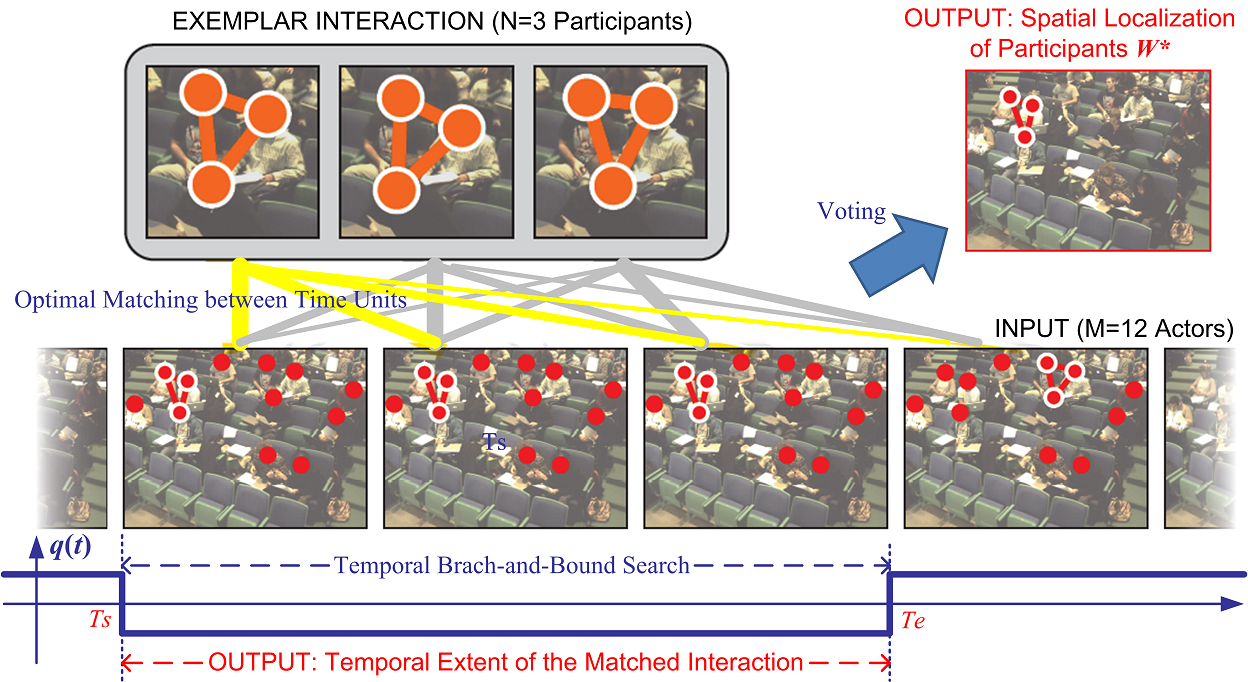
\includegraphics[width=\columnwidth]{diagram2.png}
\end{center}
\caption{Detecting and localizing interactions in social clutter. Given an exemplar video of an $N$-person social interaction, we seek to find similar interactions in a long input video with $M>N$ approximately-tracked actors. For each temporal frame in the exemplar, the $N$ best-matching participants are identified separately in each input video frame, and the matches are assigned scores. Matching scores are accumulated over time through Hough voting that is insensitive to tracking errors and changes in action rates, and this produces a spatial localization of the $N$ participating actors. Their interaction is then localized in time using an efficient branch-and-bound search.}
\label{diagram}
\end{figure}

We consider group interactions broadly as any distinctive space-time structural co-occurrence of individual actions, which occur in a variety of places and over a variety of times scales. We might want to find at a cocktail party, for example, all three-person conversations dominated by one person for a sustained period of time. On a busy street, we could search for all cases in which two passersby exchange a ``hello''. In a collection of hockey games, we might want all instances of a ``three-on-one'', and in nature we might be interested in localizing instances of distinctive group interactions among populations of animals, insects, or bacteria. Each of these cases would likely require distinct algorithms for detecting and tracking the actors, and each would benefit from action descriptors that are tuned for that setting. But beyond this, all of these scenarios can be abstracted as collections of (possibly fragmented and noisy) trajectories with accompanying time-varying action descriptors, and this is the abstraction on which we operate.
 
As depicted in Fig.~\ref{diagram}, our approach is based on matching. Given an exemplar video of a distinctive group interaction involving a small handful ($N$) of people, we aim to detect and localize instances of similar interactions within a long video of a larger gathering (\ie, of $M\ge N$ people). We represent a group interaction as an ensemble of two types of time-varying descriptors: per-actor descriptors that encode the appearance and/or motion of each participant, and relative pairwise descriptors that encode the appearance and/or motion of each participant relative to another. Matching an exemplar interaction then amounts to searching through space and time for ensembles that are similar in some sense. This approach avoids generating explicit semantic descriptions of group interactions, and it is advantageous when one lacks the vocabulary to precisely describe a class of interactions, or when they cannot easily be broken down according to any pre-defined grammar. To use our matching approach for recognition, we simply match an input video against a labeled gallery of exemplars and then extract a class label or ranked list of labels from the resulting scored matches.

In designing our detection system we face two main challenges. First, we expect tracks to be fragmented and noisy, and we expect the presence of outlying fragments caused by false detections, so we want an approach that can succeed in spite of these. Second, we expect that the same type of interaction can occur over different temporal extents, and at variable rates within its temporal extent, so we want an approach that is insensitive to these ``within-class'' variations. We address these challenges using a voting-based approach, which is depicted in Fig.~\ref{diagram}. First, the social descriptor-ensemble at each exemplar time frame is compared separately to each frame of the input video, and the best-matching $N$ participants in each frame are identified along with their matching score (yellow and gray lines in Fig.~\ref{diagram}). Second, weighted votes are accumulated from these frame-wise matches to obtain a final estimate of the $N$ participants. Third and finally, the temporal extent of the interaction is determined through an efficient branch-and-bound search. Our designs for these three processing stages are tightly connected to each other and to our representation for interactions. Optimal frame-wise matching is made possible by our restriction to second order (individual and pairwise) action descriptors, and a large-margin-based metric learning procedure serves the dual role of improving frame-wise matching (step one) and enabling efficient branch and bound search (step three).

Previous work on action detection mostly consider actions of a single actor~\cite{Ke:detection,Yuan:detection,Shechtman:detection,Hu:detection,Laptev:detection,Duchenne:detection}. Previous work on group activity recognition 1) both assume an input video to be temporally cropped around one group activity and assume no by-standers \cite{Intille:act,Ni:group,Lan:Group}; 2) only account for temporal localization \cite{Hongeng:act,Gong:act,Hakeem:act,McCowan:meeting,Choi:recogtrack,Vlad:group, Ryoo:group, CRIM13}; or 3) only consider identifying participants \cite{Li:segmentation,Cristani:discovery}. We build upon \cite{Amer:group} which address a similar problem to ours but with less flexible representations of social interactions (more on this in Section~\ref{expall}). 

We evaluate our approach using three very different datasets: 1) the UT-Interaction Dataset~\cite{Ryoo:group}; 2) a new collection of videos from an `interactive classroom' (e.g.~\cite{Crouch:PI}) in which students self-organize in small group discussion; and 3) the Caltech Resident-Intruder Mouse dataset \cite{CRIM13}.



%Each detected instance of interaction is spatially localized in that the $N$ participants are distinguished from the $M-N$ bystanders and explicitly identified with the participants in the exemplar video. Each detected instance is also temporally localized by inferring the exact times in which the interaction begins and ends. 
%So our approach operates primarily in the space of tracklets, with a critical design criteria being insensitivity to tracking errors (\eg, broken tracks and false tracklets) in the input video.

%Our work builds on a small collection of related work: \cite{Li:segmentation} identifies the relevant motion from a clutter, \cite{Cristani:discovery} detects pre-defined geometric configuration of individual poses, and \cite{Lan:retrieval} retrieves individual actions in the context of surrounding humans. Those more similar to ours are \cite{Ryoo:group,Amer:group}: The former recognizes and temporally localizes interactions, and the latter implicitly infers participants from a generative model for a set of histograms of pose-coded detections computed at a dense spatio-temporal grid. We empirically compare our approach with \cite{Ryoo:group,Amer:group} in Section \ref{expall}.


%In a round-table discussion, we could find intervals where one speaker holds the attention of her neighbors for some extended time. 